\documentclass[11pt]{article}
\usepackage[T1]{fontenc}
\usepackage{lmodern,microtype}
\usepackage[a4paper,margin=24mm]{geometry}
\usepackage{amsmath,amssymb,graphicx,booktabs,array,xcolor}
\usepackage[colorlinks=true,urlcolor=blue!45!black]{hyperref}
\hypersetup{pdftitle={Why centering helps a random matching},pdfsubject={An illustrated reading guide for problem 21}}
\usepackage{enumitem}
\setlist{itemsep=5pt,topsep=6pt}
\definecolor{ink}{HTML}{26394B}
\definecolor{teal}{HTML}{176B8A}
\definecolor{rust}{HTML}{BB5B28}
\newcommand{\E}{\mathbb E}
\newcommand{\shc}{\operatorname{sinhc}}
\newcommand{\pagetitle}[2]{\noindent{\small\sffamily\color{teal}#1}\par\vspace{5pt}\noindent{\LARGE\bfseries\color{ink}#2}\par\vspace{12pt}}
\setlength{\parindent}{0pt}
\setlength{\parskip}{7pt}
\begin{document}
\pagetitle{PROBLEM 21 / READING GUIDE}{Why centering helps a random matching}

A permutation matrix records a random one-to-one matching. Every row and every column contains exactly one entry equal to one. All other entries are zero.

Subtracting the mean $1/N$ from an entry is called \emph{centering}. The question is what happens when we multiply many such entries and take the expectation. This is the small probabilistic calculation hidden inside much larger spectral-gap proofs.

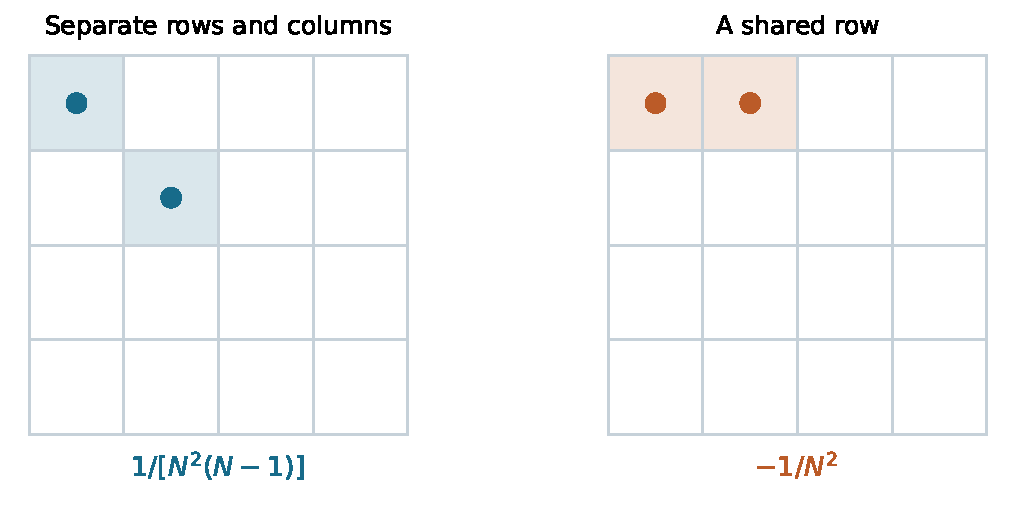
\includegraphics[width=\textwidth]{../figures/cell-patterns.pdf}

The dots show the two requested cells, not a realized permutation. For cells in different rows and columns,
\[
\E[(M_{11}-1/N)(M_{22}-1/N)]
=\frac1{N(N-1)}-\frac1{N^2}
=\frac1{N^2(N-1)}.
\]
For cells sharing a row, both indicators cannot equal one. Their centered product instead has expectation $-1/N^2$.

\textbf{The lesson.} Separate cells gain an extra factor of about $1/N$. Conflicting cells do not. Taking absolute values before evaluating the product would hide this cancellation.

\textbf{What the manuscript adds.} A direct proof handles arbitrary mixed products, including repeated cells and independent matching colors. The constant in its square-root range is optimally $\sqrt e$. For distinct diagonal cells, we also determine the exact transition scale, extend the approximation beyond that transition, and compute the next correction.

The known starting recurrence and leading terms are credited to Collins and Nagatsu. The graph application is the estimate in Bordenave's Proposition 28, imported by Brito, Dumitriu and Harris.

\newpage
\pagetitle{THE PROOF IN THREE MOVES}{Preserve cancellation until it has paid off}

Call a requested cell \emph{isolated} if no other requested cell of the same color shares its row or column. An isolated centered singleton appears once, centered, and with no uncentered copy of that cell.

\textbf{1. Set those singletons aside.} Every other cell factor is an affine expression $c+dM$, because an indicator satisfies $M^2=M$. Expanding these factors selects some matches that must occur.

\textbf{2. Condition only on compatible matches.} If $r$ selected matches have distinct rows and columns, they occur with probability $1/(N)_r$. Delete their rows and columns. The remainder is exactly a uniform permutation of size $N-r$.

The original centering is still $1/N$. For the remaining matrix $U$, set $Z=NU-1$. Every remaining row now sums to $r$. It does not sum to zero.

\textbf{3. Sum a row before taking absolute values.} Let $\mu_j$ be the expectation of the product of $j$ separated $Z$ entries. The row sum gives
\[
(N-r-j+1)\mu_j
=(r+2j-2)\mu_{j-1}+(j-1)\mu_{j-2}.
\]
For $j=1$, omit the last term. The initial values are $\mu_0=1$ and $\mu_1=r/(N-r)$. All coefficients are nonnegative.

A new column keeps all $j$ factors. A used column collides with an old factor, and the identity
\[
Z_uZ_v=-Z_u-Z_v-1
\]
removes one or two factors. This turns a cancellation problem into a positive recurrence we can bound by induction.

\textbf{The resulting estimate.} For $a$ distinct cells, $h$ isolated centered singletons and $b$ conflicting centered singletons,
\[
|\E P|\le\sqrt e\,2^bN^{-a}
\left(\frac{\sqrt{a-1}}{\sqrt N-\sqrt{a-1}}\right)^h,
\qquad 2\le a\le\sqrt N.
\]
Each isolated singleton earns an additional small factor. The exact theorem improves the prefactor to $N^{a-h}/(N)_{a-h}$. Compatible uncentered matches with $N=a^2$ show why the universal constant cannot be smaller than $\sqrt e$.

\textbf{Why the conditioning matters.} Exposing both an image and a preimage can reveal two arrows. For a permutation of four elements, knowing $2\mapsto3$ and $4\mapsto2$ leaves two choices for the image of row 1. Counting only one removed arrow would give the wrong denominator. The manuscript records this source-proof issue precisely and supplies the replacement argument above.

\newpage
\pagetitle{THE FIRST TRANSITION}{Why the order enters as a cube}

For $k$ distinct diagonal cells define
\[
a_k(N)=\E\prod_{i=1}^k(M_{ii}-1/N),\qquad R_k=a_k/L_k.
\]
The known leading terms depend on parity:
\[
L_{2m}=(2m-1)!!N^{-3m},\qquad
L_{2m+1}=\frac{4m}{3}(2m+1)!!N^{-3m-2}.
\]
We use $k\ge2$. The first centered moment is zero and has no such ratio.

The normalized even recurrence changes by order $m^2/N$ at step $m$. There are about $m$ steps, so the accumulated change has scale $m^3/N$. The odd recurrence averages these changes differently, which explains the two limits.

The proof turns that intuition into bounds:
\[
R_k-1\ge\frac{2k^3}{27N}\quad(2\le k\le N),\qquad
R_k\le e^{3k^3/N}\quad(2k\le N).
\]
Thus $R_k\to1$ \textbf{exactly when} $k^3/N\to0$. This settles the optimal-scale question posed in the published paper by Collins and Nagatsu.

At $k^3/N\to c$, the even and odd ratios tend to
\[
\cosh\left(\frac23\sqrt c\right),\qquad
\frac{\sinh(\frac23\sqrt c)}{\frac23\sqrt c}.
\]
The second value is interpreted as one at $c=0$. For $c=9/4$, the limits are about $1.543$ and $1.175$. The original leading term is no longer relatively accurate, and parity remains visible.

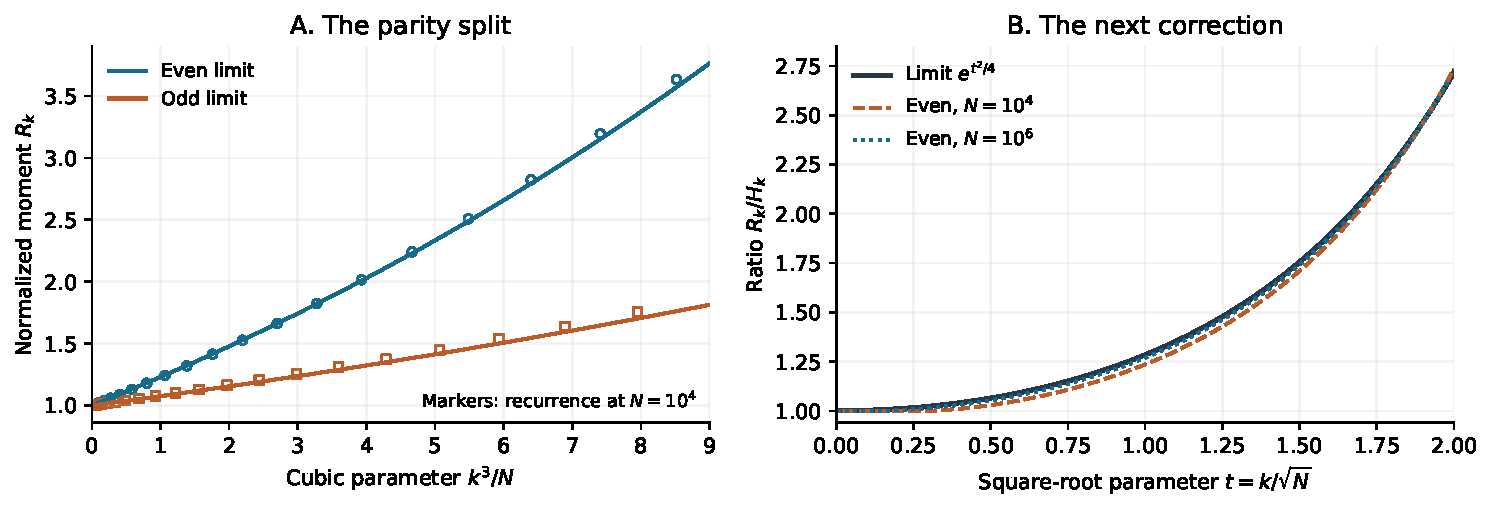
\includegraphics[width=\textwidth]{../figures/moment-regimes.pdf}

Left: the critical transition. Right: a later correction described on the next page. Markers and finite-size curves come from the positive recurrence. They illustrate the theorems rather than prove them.

\newpage
\pagetitle{THE NEW EXTENSION}{Pairs, triples and the next boundary}

Clear the denominators by setting $Q_k=(N)_kN^ka_k$. Its positive generating function is
\[
\sum_{k\ge0}Q_k\frac{z^k}{k!}
=\exp\left(N\sum_{j\ge2}\frac{j-1}{j}z^j\right).
\]
As a formal series this is a classical Laguerre identity. For the permutation application, $k\le N$. Its coefficients count weighted partitions of the $k$ labeled factors. There are no singleton blocks.

A block of size $j$ carries weight $N(j-1)(j-1)!$. A pair therefore has weight $N$, a triple has weight $4N$, and a block of four has weight $18N$.

For six factors the complete count is
\begin{center}
\begin{tabular}{llr}
\toprule
Partition shape & Number and weight & Contribution\\
\midrule
Three pairs & $15$ partitions, each $N^3$ & $15N^3$\\
Two triples & $10$ partitions, each $16N^2$ & $160N^2$\\
A pair and a block of four & $15$ partitions, each $18N^2$ & $270N^2$\\
One block of six & $1$ partition of weight $600N$ & $600N$\\
\bottomrule
\end{tabular}
\end{center}
So $Q_6=15N^3+430N^2+600N$.

\textbf{Pairs give the leading term.} The leading even contribution uses pairs only. The leading odd contribution uses one triple and otherwise pairs. Extra triples arrive with an even or odd parity restriction. Their exponential sums are precisely a hyperbolic cosine and a normalized hyperbolic sine.

Set $K=2\lfloor k/2\rfloor$, $\lambda=\frac23\sqrt{K^3/N}$ and
\[
H_k=\cosh\lambda\ \ (k\text{ even}),\qquad
H_k=\sinh\lambda/\lambda\ \ (k\text{ odd}).
\]
The extended theorem proves $R_k/H_k\to1$ throughout $k=o(\sqrt N)$. This includes orders much larger than $N^{1/3}$, where $R_k$ itself already diverges.

\textbf{Blocks of four mark the next boundary.} When $k^2/N\to d>0$, their contribution survives. The triples use a vanishing fraction of the labels, but their cumulative effect on the number of available pairings stays nonzero. Combining these effects with the permutation probability gives
\[
\frac{R_k}{H_k}\longrightarrow e^{d/4}.
\]
At $k\sim\sqrt N$, the correction is $e^{1/4}\approx1.284$. Including the factor $e^{k^2/(4N)}$ restores uniform relative accuracy for $k\le C\sqrt N$ with fixed $C$. This corrected approximation assumes that $k/\sqrt N$ stays bounded.

\newpage
\pagetitle{BACK TO GRAPHS}{What this proves for the spectral argument}

\textbf{Random lifts.} Each base edge carries an independent random permutation. Orient the base edges once, and treat each permutation as a color. The mixed-product theorem directly supplies Bordenave's Proposition 28.

\textbf{Biregular graphs.} Match the left half-edges to the right half-edges. There are
\[
L=n_Ld_L=n_Rd_R
\]
half-edges on each side, so the random block is a permutation matrix of size $L$. Its entries are centered at $1/L$. This is the input used by Brito, Dumitriu and Harris in preprint Lemma 7, published as Lemma 5.6.

\textbf{The proof chain.}
\begin{enumerate}
\item Expand powers of a non-backtracking matrix into walks that do not immediately reverse an edge.
\item Expand a high norm moment into products of matching entries.
\item Apply the mixed-product bound to each fixed pattern.
\item Count the patterns and control the contribution of local tangles.
\item Translate the non-backtracking bound back to adjacency eigenvalues.
\end{enumerate}
The manuscript proves the probability estimate in step 3 and explains the surrounding chain. The graph enumeration and tangle remainder are separate requirements.

\textbf{A concrete spectral bridge.} If the degrees are $d_L,d_R\ge2$, put $\alpha=d_L-1$ and $\gamma=d_R-1$. A positive adjacency singular value $s$ and the associated non-backtracking parameter satisfy
\[
s^2=x+\frac{\alpha\gamma}{x}+\alpha+\gamma,\qquad x=z^2.
\]
The circle $|x|=\sqrt{\alpha\gamma}$ corresponds to
\[
|\sqrt\alpha-\sqrt\gamma|\le s\le\sqrt\alpha+\sqrt\gamma.
\]
An $s$ above the upper endpoint forces a non-backtracking root outside the circle. This is why controlling those roots yields a spectral gap.

\textbf{What remains separate.} The sharper moment formulas do not automatically give a better graph eigenvalue bound. The proof does not certify every later step in the cited graph papers. The priority audit found no exact duplicate of the new quantitative refinements, but is a bounded literature search rather than a universal novelty certificate.

\vfill
{\small\color{ink}\textbf{Reading route.} Start with manuscript Sections 2 and 6 for the requested estimate and graph application. Sections 3 through 5 give the new asymptotic results. Section 7 records the two conditioning examples. Primary sources: \href{https://arxiv.org/abs/1502.04482v4}{Bordenave, Proposition 28}, \href{https://arxiv.org/abs/1804.07808v6}{Brito, Dumitriu and Harris, Lemma 7}, and \href{https://doi.org/10.5802/alco.480}{Collins and Nagatsu, Proposition 3.3 and Remarks 3.4 and 3.5}.}
\end{document}
